\chapter{La gestione della persistenza}

Nel contesto di un sistema che prevede la gestione di eventi e impegni, 
è essenziale garantire all’utente di poter accedere in qualsiasi momento alla propria agenda, 
visualizzando gli appuntamenti più urgenti e pianificando efficacemente il proprio tempo. 
Deve perciò essere possibile trovare e mostrare nel minor tempo possibile i dati relativi all’agenda. 
Per soddisfare questo requisito, 
il recupero e la visualizzazione dei dati devono avvenire con la massima rapidità possibile, 
riducendo i tempi di latenza e ottimizzando il flusso di interazione con l’interfaccia utente.\\
\\
L'adozione di un meccanismo di salvataggio locale sui dispositivi 
offre il vantaggio di migliorare le prestazioni, 
consentendo un accesso immediato alle informazioni senza dover effettuare continue richieste al server remoto. 
Tuttavia questa soluzione rimane parziale, 
in quanto non garantisce una persistenza a lungo termine dei dati,
né assicura la loro disponibilità in ogni momento, 
per essere in grado di sincronizzare più dispositivi. 
Per superare tali criticità, 
è necessario definire una strategia di gestione della memoria 
che preveda una fonte di dati centrale e autorevole, 
alla quale tutti i dispositivi possano fare riferimento per recuperare e 
aggiornare le informazioni in modo coerente e affidabile.\\
\\
Un sistema di persistenza efficace deve quindi prevedere 
un meccanismo di sincronizzazione tra i dati salvati localmente e 
la loro controparte ufficiale memorizzata nel database principale. 
Questo processo deve essere progettato in modo da garantire 
integrità, coerenza e scalabilità nelle interazioni, 
per essere resistente anche in presenza di un volume significativo di richieste concorrenti. 
La struttura del sistema di memorizzazione deve inoltre essere progettata 
tenendo conto del dominio applicativo e delle esigenze specifiche di utilizzo, 
al fine di assicurare un bilanciamento ottimale tra efficienza e robustezza operativa.\\
\\
Oltre alla gestione della persistenza dei dati per il singolo utente, 
è necessario affrontare il problema della modifica di eventi condivisi. 
Poiché l'applicazione consente a più utenti di interagire sugli stessi eventi, 
le modifiche effettuate da un partecipante devono essere propagate
in tempo reale agli altri dispositivi coinvolti. 
Questo introduce la necessità di implementare un sistema di aggiornamento distribuito, 
in grado di mantenere sincronizzati non solo i dispositivi di un singolo utente, 
ma anche quelli di tutti gli utenti interessati dalle modifiche.\\
\\
La gestione dell’accesso ai dati richiede quindi l’implementazione di un’architettura che preveda 
un punto di riferimento centrale chiaro e affidabile, 
capace di fungere da fonte primaria delle informazioni. 
Al tempo stesso, l’utilizzo di copie locali dei dati sui dispositivi client 
consente di ridurre l’impatto delle latenze di rete, 
migliorando la reattività dell’interfaccia e offrendo un’esperienza utente più fluida.
Tuttavia, questa scelta introduce la necessità di gestire due livelli distinti di responsabilità: 
da un lato, il client deve occuparsi di mantenere aggiornati i dati memorizzati localmente, 
mentre il server deve garantire la corretta distribuzione delle modifiche agli altri dispositivi interessati. 
La sincronizzazione e la gestione delle versioni dei dati diventano quindi 
elementi chiave per assicurare la coerenza del sistema e 
prevenire eventuali conflitti tra modifiche concorrenti.

\clearpage
\section{L'analisi per l'identificazione del database}

Nell’implementazione di applicazioni scalabili, la gestione del salvataggio dei dati 
può essere strutturata secondo un modello centralizzato o distribuito, 
a seconda delle esigenze di affidabilità, scalabilità e prestazioni del sistema. 
L’adozione di un’architettura di memoria distribuita offre molteplici vantaggi, 
tra cui una maggiore resilienza ai guasti di una singola fonte, 
la riduzione del carico di memoria su un'unica risorsa di archiviazione e 
una migliore scalabilità complessiva del sistema. 
Tuttavia, questa soluzione introduce una maggiore complessità infrastrutturale, 
poiché richiede meccanismi avanzati per garantire il recupero, 
l'affidabilità e la consistenza delle informazioni.\\
\\
Salvo specifici requisiti che rendano indispensabile la distribuzione totale o parziale della memoria, 
una strategia basata su un database centralizzato risulta più efficiente 
dal punto di vista prestazionale e semplifica la gestione complessiva del sistema. 
L’adozione di un’architettura centralizzata consente infatti 
di ottimizzare i tempi di accesso ai dati e ridurre la latenza delle operazioni, 
grazie a una minore complessità di sincronizzazione e 
di mantenimento della consistenza delle informazioni.\\
\\
I database non distribuiti si suddividono in due macro categorie principali: relazionali e non relazionali.\\
I database relazionali si caratterizzano per strutture dati rigide e schematizzate, 
che consentono di stabilire connessioni tra le diverse entità in tempi estremamente rapidi,
garantendo allo stesso tempo operazioni atomiche.
Viceversa, i database non relazionali offrono una maggiore flessibilità strutturale, 
permettendo l’archiviazione di dati eterogenei e adottando un accoppiamento più debole tra i vari oggetti. \\
\\
La scelta della tipologia di database più appropriata dipende direttamente
dalle esigenze specifiche del progetto.
Ogni prodotto è stato infatti realizzato per rispondere a una funzionalità specifica,
introducendo vantaggi per un determinato caso d'uso ma comportando anche punti deboli,
sia in termini di prestazioni che in termini di scalabilità.
Determinare il database più adatto alle esigenze dipende 
quindi non solo dalle proprietà intrinseche della tecnologia,
ma sopratutto di come queste riescano a risolvere i particolari problemi che il progetto presenta.
\clearpage

\subsection{Le proprietà dei database relazionali}


I database relazionali gestiscono i dati tramite strutture chiamate schemi.
Lo schema è una struttura rigida i cui campi e le relative proprietà 
vengono definite sin dal momento della creazione.
Mantengono però un grande potere espressivo, 
in quanto permettono di descrivere direttamente le relazioni(e le loro proprietà) tra gli oggetti, 
attraverso la creazione di uno schema dedicato.
Ogni elemento ha un identificativo univoco(Primary Key o PK) 
attraverso cui viene individuato all'interno del suo schema. 
Se lo schema descrive una relazione, viene identificato tramite
una combinazione di identificativi derivati(Foreign Key o FK).
Gli aggiornamenti agli schemi avvengono tramite un rigoroso sistema di transazioni.
La transazione è il processo attraverso il quale una modifica viene portata a termine,
a cui viene riservata per il tempo necessario la risorsa interessata.\\
\\
Grazie alla struttura statica dei dati, unitamente alle relazioni predefinite del dominio,
il tempo di recupero e analisi dei dati risulta altamente ottimizzato.
L'utilizzo delle primary e foreign key consente al database di creare automaticamente indici 
dedicati che consentono l'individuazione di un oggetto in tempi minimi,
e facilitano l'incrocio delle informazioni contenute all'interno delle relazioni.
L'utilizzo delle transazioni rende i database relazionali in grado di garantire 
le proprietà di Atomicità, Consistenza, Isolamento e Durabilità (ACID),
assicurando un’elevata affidabilità dei dati.\\
\\
La rigidità del modello non permette però di avere un elemento 
di uno schema che presenti proprietà diverse da tutti gli altri.
Non è quindi supportata l'aggiunta o la modifica di campi all'interno di un oggetto,
a meno di non cambiare la definizione dell'intero schema.
L'utilizzo delle transazioni introduce inoltre la necessità, durante le operazioni di scrittura,
di bloccare temporaneamente le risorse interessate,facendo fallire o aspettare altre richieste simultanee sullo stesso elemento,
potenzialmente influenzando le prestazioni complessive del sistema.\\
\\
Per poter garantire il successo di una transazione
il database deve controllare tutte le sessioni con il server,
il che comporta una limitazione al numero massimo di connessioni(e quindi richieste) contemporanee possibili.
Inoltre gli indici dipendono da tutti gli elementi del database,
e allo stesso modo gli schemi delle relazioni sono 
fortemente accoppiati con gli schemi delle entità coinvolte.
Risulta quindi arduo dividere degli elementi su più tabelle(sharding), 
operazione necessaria per la distribuzione del database su più server,
aumentando di conseguenza la complessità richiesta per essere in grado di scalare orizzontalmente.\\
\\

\subsection {Le proprietà dei database non relazionali}

I database non relazionali, noti anche come NoSQL, 
si distinguono per l'adozione di modelli di archiviazione dei dati flessibili, 
che si discostano dalla rigida struttura tabellare dei database relazionali. 
Questi modelli includono approcci chiave-valore, documento, colonnare e a grafo, 
ciascuno ottimizzato per specifiche esigenze applicative, 
come la gestione di file, dati semi-strutturati, o la rappresentazione di relazioni complesse.\\
\\
La loro caratteristica fondamentale è la capacità di salvare le informazioni in forme variabili, 
permettendo di modificare la struttura dei dati senza la necessità di riconfigurare lo schema del database. 
La vera forza dei database NoSQL, tuttavia, risiede nella loro predisposizione alla scalabilità orizzontale. 
I NoSQL sono infatti progettati per distribuire il carico su più server, 
consentendo di gestire volumi crescenti di dati e richieste semplicemente aggiungendo nuovi nodi al sistema.\\
\\
Nonostante i vantaggi in termini di scalabilità, 
i database non relazionali presentano però alcune limitazioni significative. 
La più rilevante è la rinuncia alle proprietà ACID, alla quale si contrappone, 
per favorire la disponibilità e la tolleranza ai partizionamenti, 
una consistenza finale (eventual consistency), 
dove le modifiche ai dati si propagano attraverso il sistema in un certo lasso di tempo, 
piuttosto che essere immediatamente consistenti su tutti i nodi.
Questo può portare a letture di dati "stale" (non aggiornati) in determinate circostanze, 
il che è può essere un problema per applicazioni che richiedono forte consistenza.\\
\\


\mycomment{
    Per mitigare queste limitazione alcuni database offrono strategie di strong consistency,
    indici?
    accostamento di databases?
}

\subsection{L'impatto delle relazioni delle entità sulle prestazioni}

L'aspetto determinante alla base della scelta del database 
riguarda la gestione delle relazioni tra le entità. 
È fondamentale analizzare la distribuzione delle richieste per ciascun elemento
e il carico computazionale che ogni operazione comporta. 
Tra le operazioni più costose in termini di prestazioni, 
che più ostacola e rallenta il recupero dei dati, vi è l'operazione di unione(join).
Durante l'operazione di unione vengono incrociati i dati di vari elementi 
per restituire un oggetto coerente che presenti tutte le proprietà necessarie, 
originariamente distribuite in molteplici tabelle. \\
\\
Nonostante l'esecuzione di join su database sia altamente ottimizzata
(particolarmente in quelli relazionali) e facilitata dall'utilizzo di indici,
introduce comunque carichi computazionali di grande entità che impattano
significativamente sui tempi di risposta delle richieste, 
crescendo proporzionalmente con la quantità dei dati presenti nel database. 
Per questo motivo è bene modellare il dominio nell'ottica di ridurre il più possibile 
le richieste che comportano l'incrocio di dati da tabelle diverse.\\
\\
Le relazioni tra elementi possono essere classificate in tre categorie principali: 
di tipo uno a uno, uno a molti, e molti a molti. \\
Nelle relazioni uno a uno il recupero dei dati è diretto 
e richiede uno sforzo computazionale limitato. 
Nei casi uno a molti e molti a molti il reperimento delle informazioni richiede 
spesso un'operazione di join, ed è quindi bene eseguire un'attenta valutazione 
delle tipologie di accesso per ottimizzarne le prestazioni.
Un'operazione di join è accettabile se il numero delle entità coinvolte è limitato o facilmente reperibile.
Altrimenti, una delle strategie possibili per migliorare l’efficienza delle richieste 
offerte dai database non relazionali è la denormalizzazione delle entità.\\
\\
La denormalizzazione consiste nel duplicare o incorporare dati correlati all'interno della stessa entità o documento, 
eliminando la necessità di operazioni di join complesse e costose in fase di lettura. 
Questo significa che, anziché avere tabelle separate tra due elementi e collegarle tramite chiavi esterne, 
un database denormalizzato potrebbe memorizzare direttamente 
un array dei dati del primo all'interno del documento del secondo.
Recuperare tutti i dati necessari per una determinata operazione richiede spesso 
una singola lettura da un'unica entità, e raramente un'operazione di join,
riducendo drasticamente il numero di accessi al disco e le elaborazioni computazionali. 
Questo è particolarmente vantaggioso in scenari
dove le operazioni di lettura sono molto più frequenti di quelle di scrittura.\\
\\
Per ogni dato duplicato, infatti, si introduce la complessità 
di dover garantire la coerenza di tali dati attraverso il sistema. 
Se un'informazione duplicata viene modificata in una delle sue occorrenze, 
è essenziale che tale modifica si propaghi correttamente a tutte le altre copie 
per evitare che il database contenga dati incoerenti.
Non esiste un meccanismo automatico che ne assicura la coerenza,
e la sua creazione può diventare onerosa e complessa, 
soprattutto in sistemi distribuiti e con elevato volume di scritture.\\
\\
In una relazione uno a molti, 
nel caso in cui la richiesta di quell'elemento non sia frequente 
ma sia invece importante restituire spesso gli elementi a lui collegati,
conviene copiare gli oggetti relativi all'interno dell'elemento singolo. 
L’impostazione inversa, in cui si copia il singolo all’interno dei molti elementi, 
comporterebbe l’ispezione di tutti i componenti esistenti alla ricerca di quelli che contengono l’elemento dato. 
Se però, viceversa, sono frequenti le richieste relative agli elementi multipli, e la loro relazione è importante, 
conviene copiare il singolo all'interno di detti elementi, per evitarne il recupero ogni volta.\\
\\
Nel caso molti a molti bisogna considerare ancora di più la proporzione delle richieste.
Le relazioni molti a molti vengono generalmente descritte da un terzo oggetto, 
che oltre a mantenere i riferimenti alle due entità,
descrive le proprietà della relazione.
Le scelte principali che si possono fare in questo caso sono due.
Se la lettura è sbilanciata verso uno dei due elementi della relazione,
e, allo stesso tempo, è importante che vengano restituiti gli oggetti 
che descrivono l'associazione assieme all'elemento stesso,
è bene integrare le associazioni in quell'elemento.
Altrimenti, in caso la necessità di lettura sia equiparabile da entrambe le parti,
è necessario mantenere l'associazione come documento indipendente, 
eventualmente copiando i dati richiesti per evitare 
di dover recuperare il terzo elemento della relazione.
\clearpage


\subsection{Analisi del dominio}

Il dominio descrive i componenti dell'applicazione e le loro relazioni. 
Ne vengono espresse le dipendenze, i rapporti reciproci e la cardinalità delle relazioni. 
La sua analisi, integrata con la previsione del carico delle richieste,
permette di fornire un quadro dettagliato sulle necessità relative,
per poter poi definire la tipologia delle strutture in cui salvare i dati e
le caratteristiche richieste al database.\\

\begin{figure}[htpb]
    \centering
    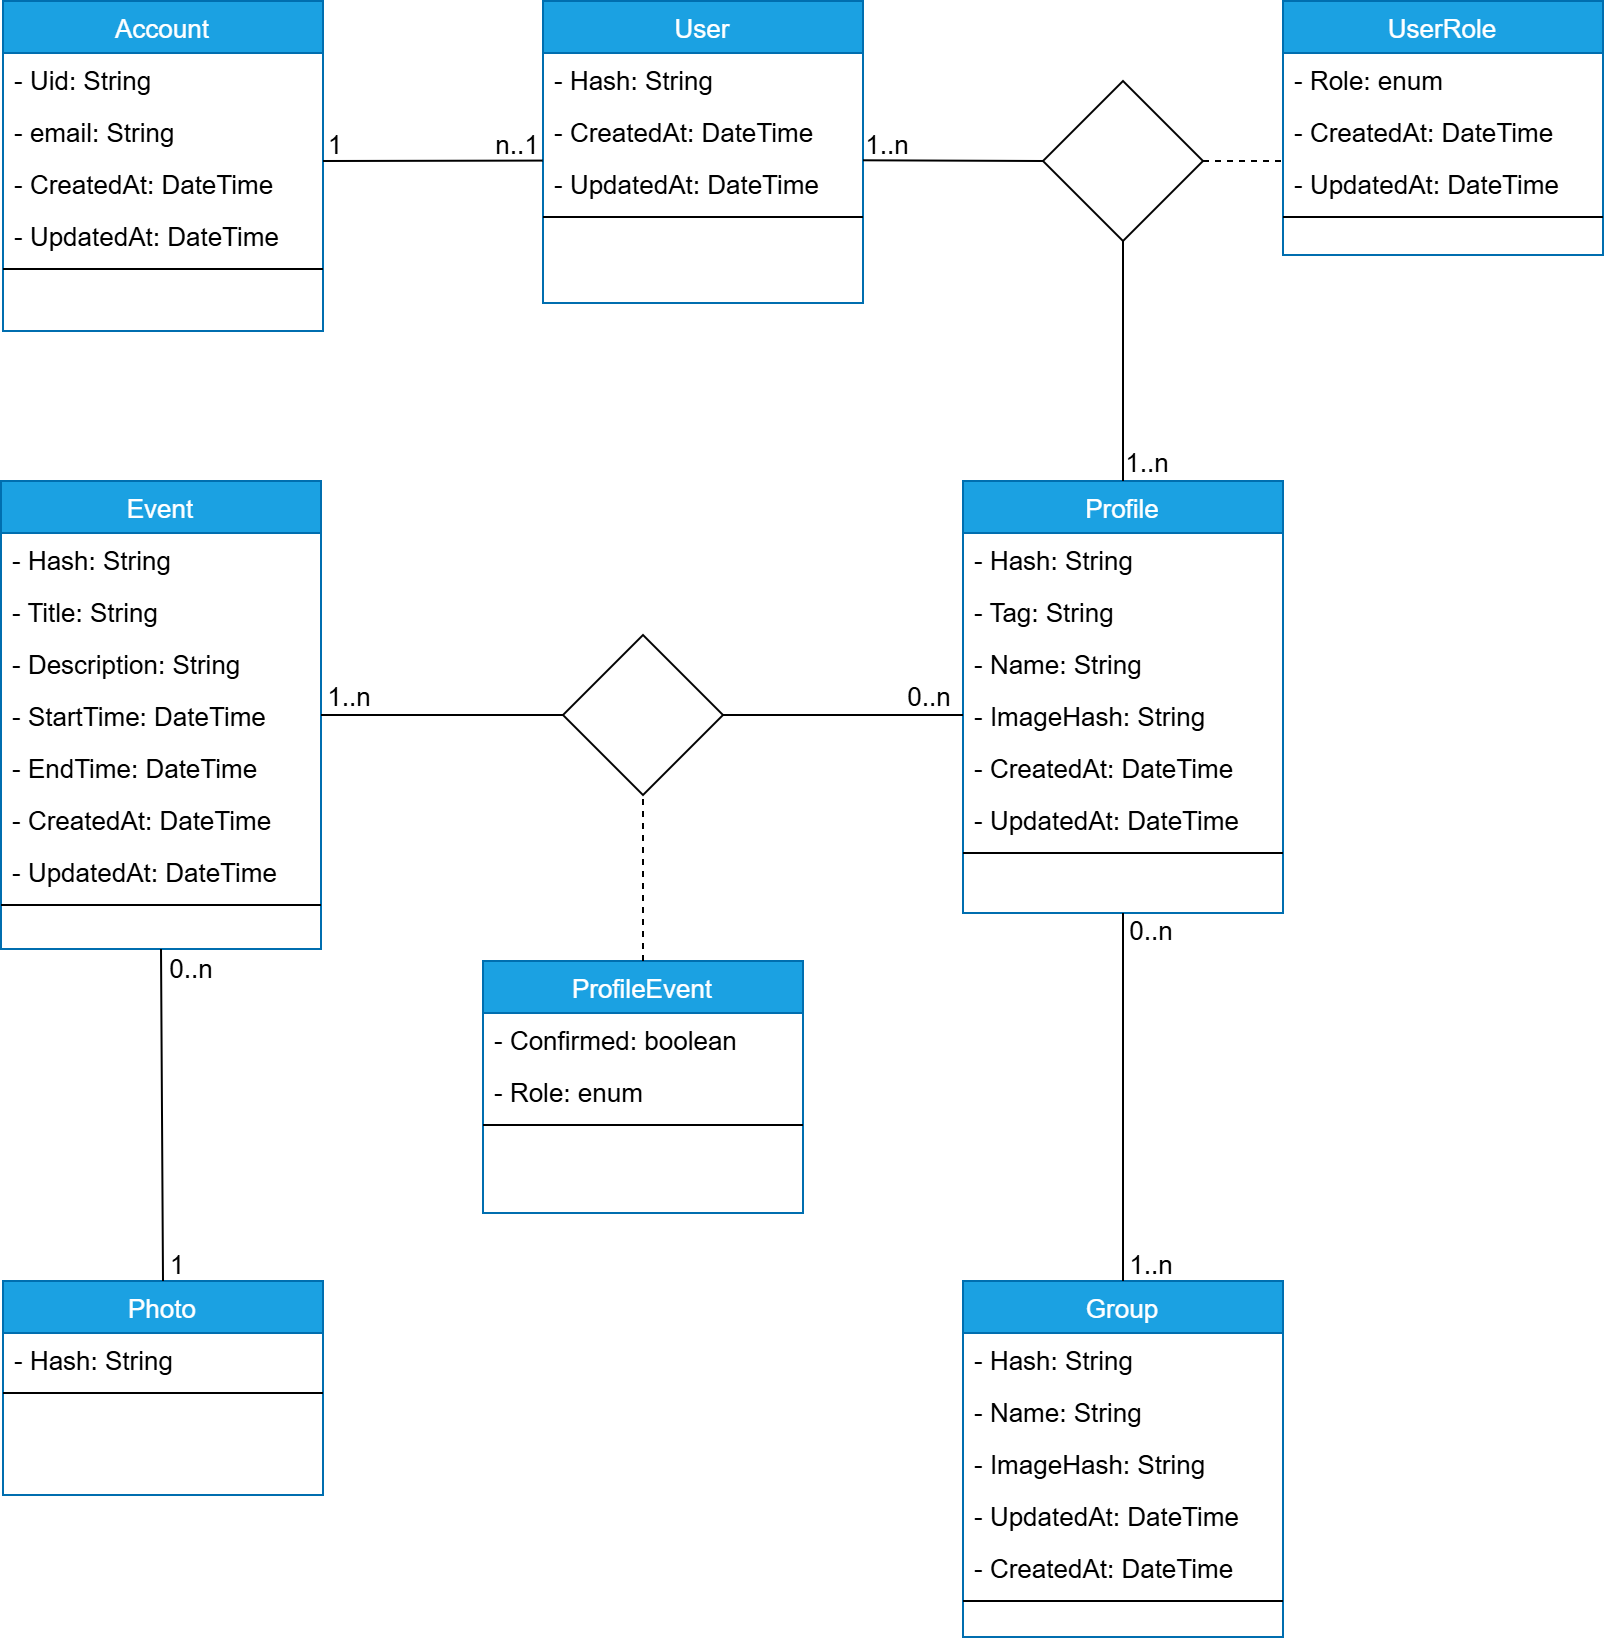
\includegraphics[width=\textwidth]{ProgettoDominioServer.png}
    \caption{Diagramma del dominio di Wyd}
\end{figure}

\clearpage
Le entità Account, User e Profile, assieme alla relazione UserRole, 
descrivono le specifiche di autenticazione, identificazione dell'utente e i suoi ruoli sui profili associati.
I loro dati vengono recuperati solamente una volta nel ciclo di vita del programma, 
a seguito del login dell'utente.
Vengono poi salvati in memoria locale, 
riducendo il numero di richieste relative successive a un controllo su eventuali aggiornamenti.
Si prevede che le modifiche a questi elementi siano sporadiche.\\
Allo stesso modo gli oggetti Group vengono recuperati solo all'avvio dell'applicazione, e, 
salvo rari aggiornamenti, non comportano ulteriori richieste.
Le richieste di lettura e scrittura previste per questi elementi sono quindi in quantità esigua, 
e influiscono secondariamente sulle performance del sistema.\\
\\
La maggioranza delle richieste verterà sull'ottenimento dei dati relativi agli Event e ai Profile. 
Gli Event descrivono gli impegni ai quali i profili partecipano.
Essendo la loro relazione di tipologia molti a molti,
si introduce l'entità ProfileEvent che descrive l'associazione evento-profilo,
indicando che un evento è condiviso con un profilo.
La proprietà più importante di ProfileEvent è sicuramente Confirmed,
una variabile booleana che esprime la partecipazione o meno di un profilo all'evento.
È ragionevole prevedere che la cardinalità dei profili associati a un evento non superi l'ordine delle centinaia.
Agli eventi che si associano ai profili l'ordine di grandezza invece previsto risiede nelle migliaia. 
Ci sono molteplici situazioni da tenere in considerazione analizzando questa relazione.\\
\\
Sicuramente bisogna considerare il recupero specifico delle entità Event e Profile.
Questo accade quando un utente decide di entrare nel dettaglio di uno dei due elementi,
comportando la richiesta di tutti i dati dell'oggetto.
Consistono in un'operazione di lettura tutto sommato semplice:
essendo l'utente in possesso dell'identificativo dell'elemento,
la ricerca risulta diretta, e i dati da recuperare esigui.\\
\\
La conferma o la disdetta a un evento vede la modifica di un ProfileEvent.
Questa operazioni di per sé risulta veloce 
in quanto necessita di recuperare un solo elemento per poi modificarlo.
Allo stesso modo la modifica di un evento comporta l'aggiornamento di un solo oggetto Event,
a seguito però del recupero del ProfileEvent associato, 
necessario per controllare i permessi del profilo sull'evento.
Entrambe le operazioni richiedono però l'invio di una notifica verso tutti i profili interessati,
che necessita il recupero di tutti i ProfileEvent associati ogni volta che una di queste accade.\\
\\
La probabilità che un evento o un qualunque ProfileEvent a esso associato 
venga modificato risulta quindi complessivamente elevata e, di conseguenza,
l'operazione di recupero degli identificativi di tutti i profili associati all'evento
è da considerarsi frequente.
Questa operazione, in base all'implementazione, può risultare costosa:
una separazione, un accoppiamento debole o la mancanza di indici tra Event e ProfileEvent
determinano la necessità di ricercare le entità in tutto il database.\\
\\
Quando un utente accede per la prima volta su un dispositivo 
è necessario ottenere gli eventi associati ai suoi profili.
Allo stesso modo, a ogni avvio dell'applicazione si recuperano gli eventi
che hanno subito modifiche dall'ultimo accesso.
Inoltre, per poter garantire(all'interno di un determinato vincolo temporale) 
la consistenza dei dati anche a livello locale, 
il client applica una strategia di long polling 
per ottenere gli eventi che sono stati modificati dall'ultimo aggiornamento noto.
L'operazione di ritrovamento degli eventi a partire dal profilo risulta quindi centrale e frequente,
per quanto possa accettare un tempo di esecuzione leggermente più lungo. \\

\begin{longtable}{|P{9.5cm}|P{2.5cm}|P{2.5cm}|}
    \hline
    \textbf{Funzionalità} & \textbf{Frequenza }                                                 & \textbf{Complessità}\\
    \hline
    Recupero di un Event                & Media                            & Semplice                     \\
    \hline
    Recupero di un Profile         & Media                     & Semplice                     \\
    \hline
    Modifica di un Event      & Media                          & Semplice                      \\
    \hline
    Conferma/disdedda di un Event       & Alta                           & Semplice                    \\
    \hline
    Ritrovamento dei Profile associati a un Event        & Alta                           & Complessa      \\
    \hline
    Ritrovamento degli Event associati a un Profile      & Alta                          & Complessa            \\
    \hline
    \caption{Funzionalità principali tra Event e Profile}
\end{longtable}

La relazione tra Event e Photo impatta sulle prestazioni del sistema solo in casi particolari e
verrà affrontato nei capitoli successivi.
\clearpage



\section{L'implementazione del database}
Nelle sezioni precedenti si è discusso delle proprietà
offerte dai diversi tipi di database e 
delle necessità che il dominio impone sul sistema.
La scelta del database deriva quindi dall'incrocio di tutte queste condizioni,
individuando la tecnologia che meglio riesce a rispondere alle esigenze del progetto. 
Ogni tipologia di database comporta un approccio differente alle informazioni,
implicando una strategia di salvataggio e manipolazione dei dati propria.
Le strutture che modellano le entità devono quindi
essere create per sfruttare nella maniera più efficiente possibile
i vantaggi offerti dalla tecnologia scelta.\\
\\
Una volta scelto il database e le strutture in base alla modalità 
che più si addicono alle esigenze del progetto,
l'utilizzo di servizi in cloud comporta una maggiore attenzione anche 
alle proprietà legate al mantenimento del servizio,
dalle quali derivano le proprietà di scalabilità e affidabilità.
La grande differenza tra i vari servizi sta nelle proprietà del server 
incaricato di fornire il potere computazionale necessario per l’esecuzione. 
L’architettura del server e la sua integrazione con la tecnologia del database
determinano infatti l’effettiva capacità di scalabilità del servizio.\\
\\
Si intende scalabilità verticale la capacità di aumentare le risorse 
della stessa macchina in cui si esegue il codice. 
La scalabilità verticale viene definita nel momento di creazione del servizio, 
in cui si determinano le risorse da dedicare alla macchina che esegue il programma. 
Trattandosi di macchine virtualizzate, 
è sempre possibile in un secondo momento aumentare le prestazioni in caso di necessità.\\
\\
Per scalabilità orizzontale si intende invece la capacità di 
delegare il carico di lavoro ad altre macchine, eventualmente coordinando le modifiche. 
Questo permette una risposta alle richieste più resistente, 
riducendo il rischio di colli di bottiglia che potrebbero venirsi a formare nell’utilizzo di un nodo singolo.
La scalabilità orizzontale richiede però l'implementazione 
di tecnologie apposite integrate con il database che permettano l'esecuzione in nodi fisici differenti. \\
\\
Una volta individuata la tecnologia adatta e il livello di scalabilità desiderati, 
è bene considerare le altre necessità o le opportunità aggiuntive generate 
dalla presenza di un database nel progetto. \\
\\
L’alta disponibilità(HA) è la proprietà di garantire l’accesso al servizio nonostante i guasti. 
Ad esempio, si può mantenere una macchina identica al server principale in grado di replicare il servizio, 
spostando il carico in caso di guasto del server principale. 
Si misura in “numero di nove”, ovvero la quantità di nove presenti 
nella percentuale del tempo per il quale si garantisce la disponibilità del servizio.
I servizi offrono diverse qualità di HA, in base alle funzionalità desiderate.\\
\\
Alcuni servizi possono presentare offerte di backup 
per riportare il server nello stesso stato di qualche momento precedente.
Questo permette il ripristino del sistema a un punto precedente 
rispetto all'avvenimento di eventuali errori o guasti del sistema.\\
\subsection{La scelta del database}

Viste le necessità del progetto in ambito di scalabilità 
e le caratteristiche del dominio,
si individua nei database documentali la tecnologia più adatta 
per gestire la persistenza centrale dell'applicazione.\\
\\
I database documentali, facenti parte della categoria dei database non relazionali, 
rappresentano un paradigma di gestione dei dati
che organizza le informazioni in documenti. 
Ogni documento è un'unità autonoma che incapsula la descrizione di un'entità, 
contenendo le sue proprietà. 
Tali documenti sono logicamente raggruppati in collezioni.
All'interno di una collezione, 
ciascun documento è univocamente identificato da un proprio identificativo, 
garantendo l'accesso diretto e la manipolazione individuale.\\
\\
Un aspetto distintivo e strategicamente rilevante dei database documentali è
la loro intrinseca capacità di supportare la scalabilità orizzontale in modo nativo. 
Questo è un vantaggio fondamentale in architetture distribuite e ambienti ad alta intensità di dati. 
La scalabilità è realizzata attraverso la partizionamento (o sharding), 
un meccanismo che distribuisce automaticamente i dati tra diversi nodi di archiviazione fisici.\\
\\
Attraverso la denormalizzazione si possono migliorare le prestazioni di lettura, 
aggregando dati correlati all'interno di un singolo documento o partizione. 
Questo approccio semplifica la gestione delle join, 
che possono essere ottimizzate per risiedere all'interno della stessa partizione o 
in partizioni vicine, minimizzando la necessità di operazioni di lettura tra nodi distinti.\\
\\
La denormalizzazione comporta intrinsecamente 
alcune sfide a livello di consistenza dei dati, 
in particolare per le operazioni di recupero che coinvolgono dati potenzialmente duplicati. 
Questo problema è efficacemente mitigato dall'adozione di Global Secondary Indexes (GSI). 
I GSI consentono di interrogare i dati su attributi che non sono la chiave primaria del documento, 
e risiedono quindi su partizioni differenti.
Forniscono percorsi di accesso alternativi e performanti sull'intero dataset distribuito, 
superando le limitazioni imposte dalla distribuzione fisica delle partizioni e 
mantenendo un'elevata efficienza nelle query complesse.\\
\\
Implementando automaticamente e nativamente la scalabilità orizzontale,
il database relazionale ci permette quindi di gestire con efficienza 
l'incremento dei volumi di dati e dei carichi di lavoro senza interventi complessi.
Fornisce inoltre un supporto diretto all'esigenza dell'architettura 
riguardo alla necessita di letture performanti 
da entrambi i lati di relazioni molti-a-molti:
attraverso il partizionamento strategico, 
i dati correlati possono essere collocati in partizioni vicine 
per ottimizzare le letture da un lato della relazione, 
mentre i Global Secondary Indexes (GSI) superano le limitazioni delle partizioni fisiche, 
consentendo interrogazioni efficienti e performanti dall'altro lato. 
Infine, un'attenta progettazione del modello di dati, 
che include una denormalizzazione strategica e l'utilizzo degli indici, 
garantirà un tempo di recupero ridotto per le informazioni, 
massimizzando la reattività del sistema e l'efficienza complessiva.\\
\\
Un confronto con il paradigma relazionale evidenzia le ragioni della sua esclusione per le esigenze del nostro progetto. 
Sebbene i database relazionali siano soluzioni consolidate per la gestione di dati strutturati, 
presentano delle limitazioni che non si allineano con i requisiti di scalabilità richiesti. 
La loro architettura, che spesso lega indici e tabelle alla stessa partizione logica, 
impone intrinsecamente dei vincoli sulla scalabilità orizzontale, 
non solo per la difficoltà di distribuire indici e tabelle su nodi diversi, 
ma anche per il numero massimo di connessioni contemporanee che possono gestire, 
limitando la capacità di rispondere a un numero massiccio di richieste simultanee.  
L'implementazione dello sharding, sebbene possibile, è interamente a carico dello sviluppatore, 
introducendo un significativo onere di progettazione, sviluppo e manutenzione.\\
\\
Inoltre, la gestione di relazioni molti-a-molti nel modello relazionale, 
pur essendo logicamente chiara con tabelle di giunzione, 
può presentare problemi di scalabilità in contesti di elevato carico. 
Quando una query necessita di recuperare dati da entrambi i lati di una relazione molti-a-molti, 
ciò implica l'esecuzione di join complesse tra più tabelle. 
Sebbene queste operazioni possano essere veloci su singole istanze di database ben ottimizzate, 
in un ambiente distribuito e con volumi di dati in crescita, 
queste join possono richiedere il trasferimento di grandi quantità di dati tra nodi diversi per essere risolte, 
introducendo latenza e overhead di rete significativi. 
Questo può diventare un collo di bottiglia, compromettendo le performance complessive. 
Infine, la mancanza di un supporto nativo per indici secondari globali (GSI) 
rende più complessa la gestione di query su attributi non chiave distribuiti su diverse partizioni, 
costringendo a soluzioni alternative che potrebbero compromettere 
la reattività del sistema e aumentare la complessità del codice. 
Questi fattori combinati ci hanno portato a escludere il modello relazionale.\\
\\
Essendo il progetto già improntato sulla piattaforma Azure,
la ricerca verte inizialmente tra le opzioni che mette a disposizione.
Azure offre un’ampia scelta di database documentali che possono essere integrati con il resto dell’ecosistema. 
Tuttavia, Azure presenta un servizio completamente gestito e nativo
per i database non relazionali chiamato Azure Cosmos DB.
Garantendo la massima interoperabilità all'interno dell'ecosistema,
si procede analizzando le proprietà e i vantaggi offerti da Cosmos DB.\\
\\
Azure Cosmos DB si distingue per la sua capacità di scalare orizzontalmente in maniera illimitata, 
consentendo di gestire volumi di dati e carichi di lavoro molto elevati, 
fino a milioni di richieste al secondo, 
grazie alla possibilità di distribuire il carico à su più regioni Azure. 
È stato infatti ideato per essere presentare un'architettura distribuita, 
con replica automatica dei dati, 
assicurando un'elevatissima disponibilità e resilienza. 
Queste vengono assicurate anche in caso di interruzioni regionali, 
grazie a meccanismi di failover automatico.
Inoltre, la distribuzione globale "turnkey" garantisce che i dati siano sempre vicini agli utenti, 
riducendo drasticamente la latenza a millisecondi a cifra singola 
(con SLA del 99.999\% di disponibilità per account multi-regione).
Consente l'indicizzazione attraverso più partizioni in maniera 
automatica e personalizzabile ottimizzado le query, 
riducendo la complessità e migliorando le prestazioni, 
senza richiedere oneri di gestione manuale degli indici.\\
\\
Pur essendo focalizzato sui database documentali,
Cosmos DB è però una soluzione multi-modello e multi-API. 
Supporta infatti, oltre alla sua API nativa per NoSQL (che usa il modello a documenti JSON), 
anche API compatibili con MongoDB, Apache Cassandra, Apache Gremlin (per i grafi) e Azure Table. 
Questa versatilità permette agli sviluppatori di utilizzare strumenti familiari, 
semplificando la migrazione di applicazioni esistenti o 
lo sviluppo di nuove con la flessibilità di scegliere il modello di dati più appropriato.\\
\begin{figure}[h!]
    \centering
    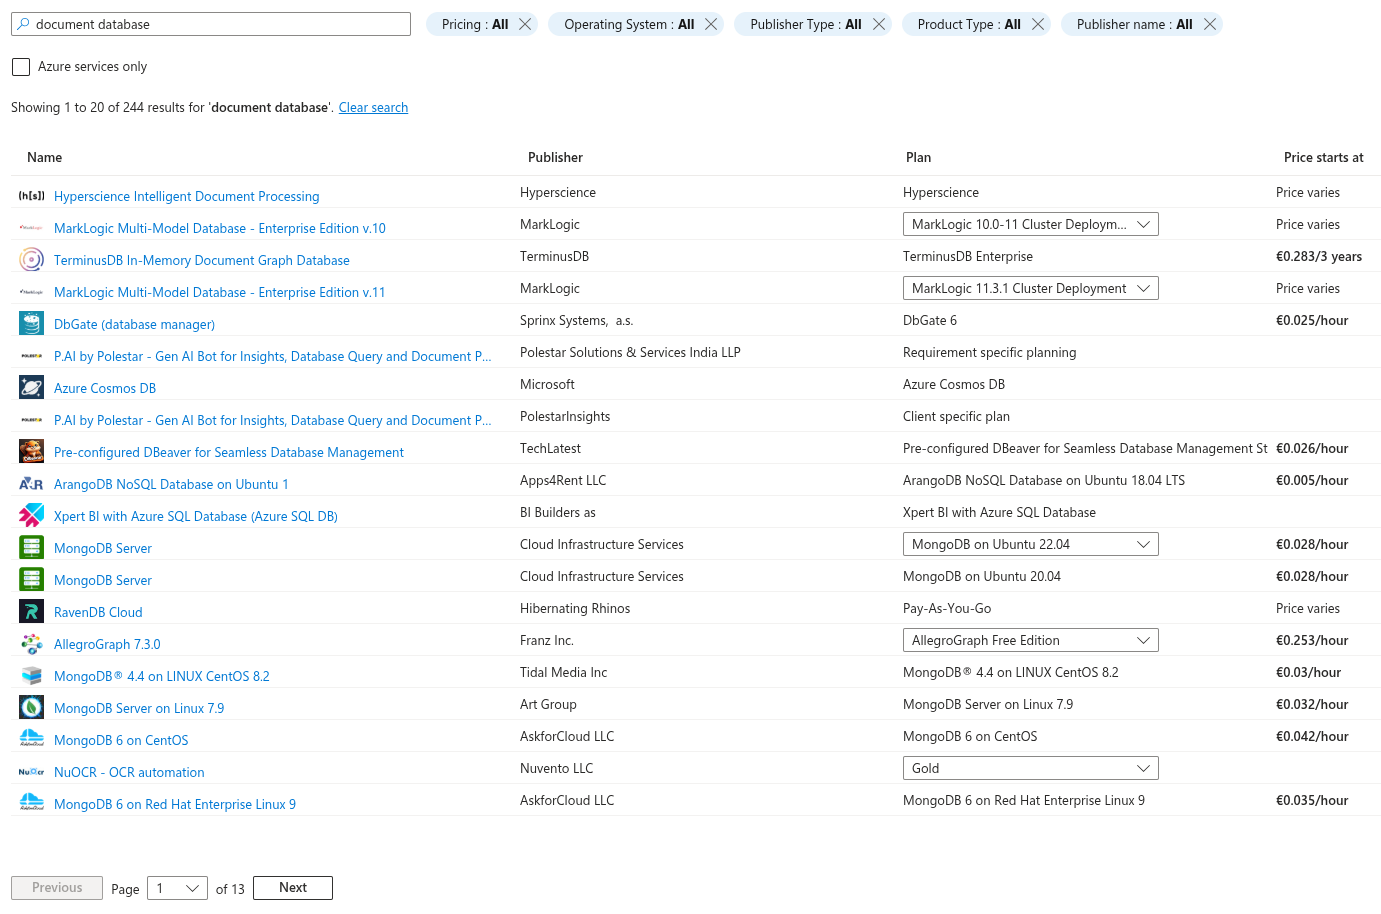
\includegraphics[width=\textwidth]{AzureDatabase.png}
    \caption{Proposte di Azure per i database documentali}
\end{figure}

A livello di costi è difficile fare un'analisi precisa,
in quanto tutti i competitor presentano modelli di pagamento che utilizzano metriche di utilizzo diverse,
rendendo necessarie ulteriori analisi che dipendono anche 
dall'effettivo numero e tipologie di richieste che vertono sul database.
Di seguito viene riportata una tabella per comparazione i costi delle alternative principali.
Cosmos usa come metrica le Rerquest Units(RU) per quantificare l'impatto di una richiesta sul database.
Le RU rappresentano un'astrazione delle risorse di sistema (CPU, I/O, memoria) necessarie per eseguire tali operazioni.\\
\\
\begin{longtable}{|P{9.5cm}|P{2.5cm}|P{2.5cm}|}
    \hline
    \textbf{Servizio} & \textbf{Costo ogni milione di scritture (normalizzate a 1 KB) }                                                 & \textbf{Costo ogni milione di scritture (normalizzate a 1 KB) }\\
    \hline
    AWS DynamoDB               & \$1.25                            & \$0.25                     \\
    \hline
    Google Cloud Firestore         & \$0.90                     & \$0.30                    \\
    \hline
    Azure Cosmos DB      & In base al consumo di RU, \$5.84 al mese ogni 100RU/s    & In base al consumo di RU, \$5.84 al mese ogni 100RU/s                       \\
    \hline
    MongoDb Atlas       & Varia in base all'host                          & Varia in base all'host                    \\
    \hline
    \caption{Funzionalità principali tra Event e Profile}
\end{longtable}

Inoltre, Azure mette a disposizione molteplici servizi accessori che possono essere uniti al servizio. 
Questo permette di estendere le potenzialità del database tramite  l’analisi e il monitoraggio dei dati, 
generando prestazioni aggiuntive o integrando i dati per lo sviluppo di altre tecnologie.\\
\\

Al server principale è stata affiancata una replica che rimane costantemente aggiornata. 
Situata in una località differente dal server principale, 
garantisce alta disponibilità continuando a fornire i servizi anche in caso di malfunzionamenti al server principale.\\
\\

Nel caso in cui però fossero necessarie ulteriori prestazioni, 
se il dominio e i requisiti lo permettono, 
si può eventualmente delegare a un database non relazionale le modifiche ai dati e alle relazioni 
che non necessitano delle qualità ACID ma richiedono un’alta frequenza di scrittura.\\
\\ 
Interporre una cache tra la logica applicativa e il database
semplifica e riduce il numero di richieste verso il database. 
Il livello di caching si occupa di gestire le richieste al database 
fornendo e duplicando le risposte che possiede già in memoria, 
eventualmente concentrando le richieste in caso i dati siano invece da recuperare. 
Per i dati in scrittura, invece, salva temporaneamente le modifiche richieste, 
aggiornando subito la memoria locale, 
per poi apportare le modifiche al database in momenti di carico ridotto. 
Garantisce così un tempo di risposta e di propagazione degli aggiornamenti ridotto,
alleviando il numero di richieste al database, estendendo così  le prestazioni fornite.\\
\\


Tuttavia, non vi è alcun vincolo che impedisca l'affiancamento di database di tipologia diversa 
per rispondere a esigenze specifiche e sfruttare i punti di forza di entrambe le tecnologie.
\\

\subsection{La definizione delle classi}
Nonostante sia più probabile che venga richiesto il dettaglio di un evento, 
e quindi sia più frequente il dover recuperare i Profile relativi all’Event, 
la proporzione delle richieste prevista non giustifica lo sbilanciamento della relazione sugli Event.
Infatti, se si salvassero tutti i ProfileEvent sull’oggetto Event, 
le richieste degli eventi appartenenti ai profili, sebbene meno frequenti, 
richiederebbero l’ispezione di tutti gli Event alla ricerca del Profile indicato. 
Infine, se si duplicasse l’oggetto ProfileEvent, 
oltre che nella sua tabella originaria, anche sugli Event la sua creazione, 
la sua eliminazione e la modifica del campo Confirmed richiederebbero il doppio delle scritture.\\
\\



\subsection{L'integrazione con le Azure Functions: il framework .Net e l'eventual consistency}

\clearpage




\clearpage




\subsection{L' integrazione con C\#}

La scelta di un database relazionale per la persistenza ha comportato sviluppi progettuali precisi. 
In primis si rende necessario tradurre il dominio in componenti relazionali che possano essere espressi e salvati nelle tabelle del database.

\begin{figure}[h!]
    \centering
    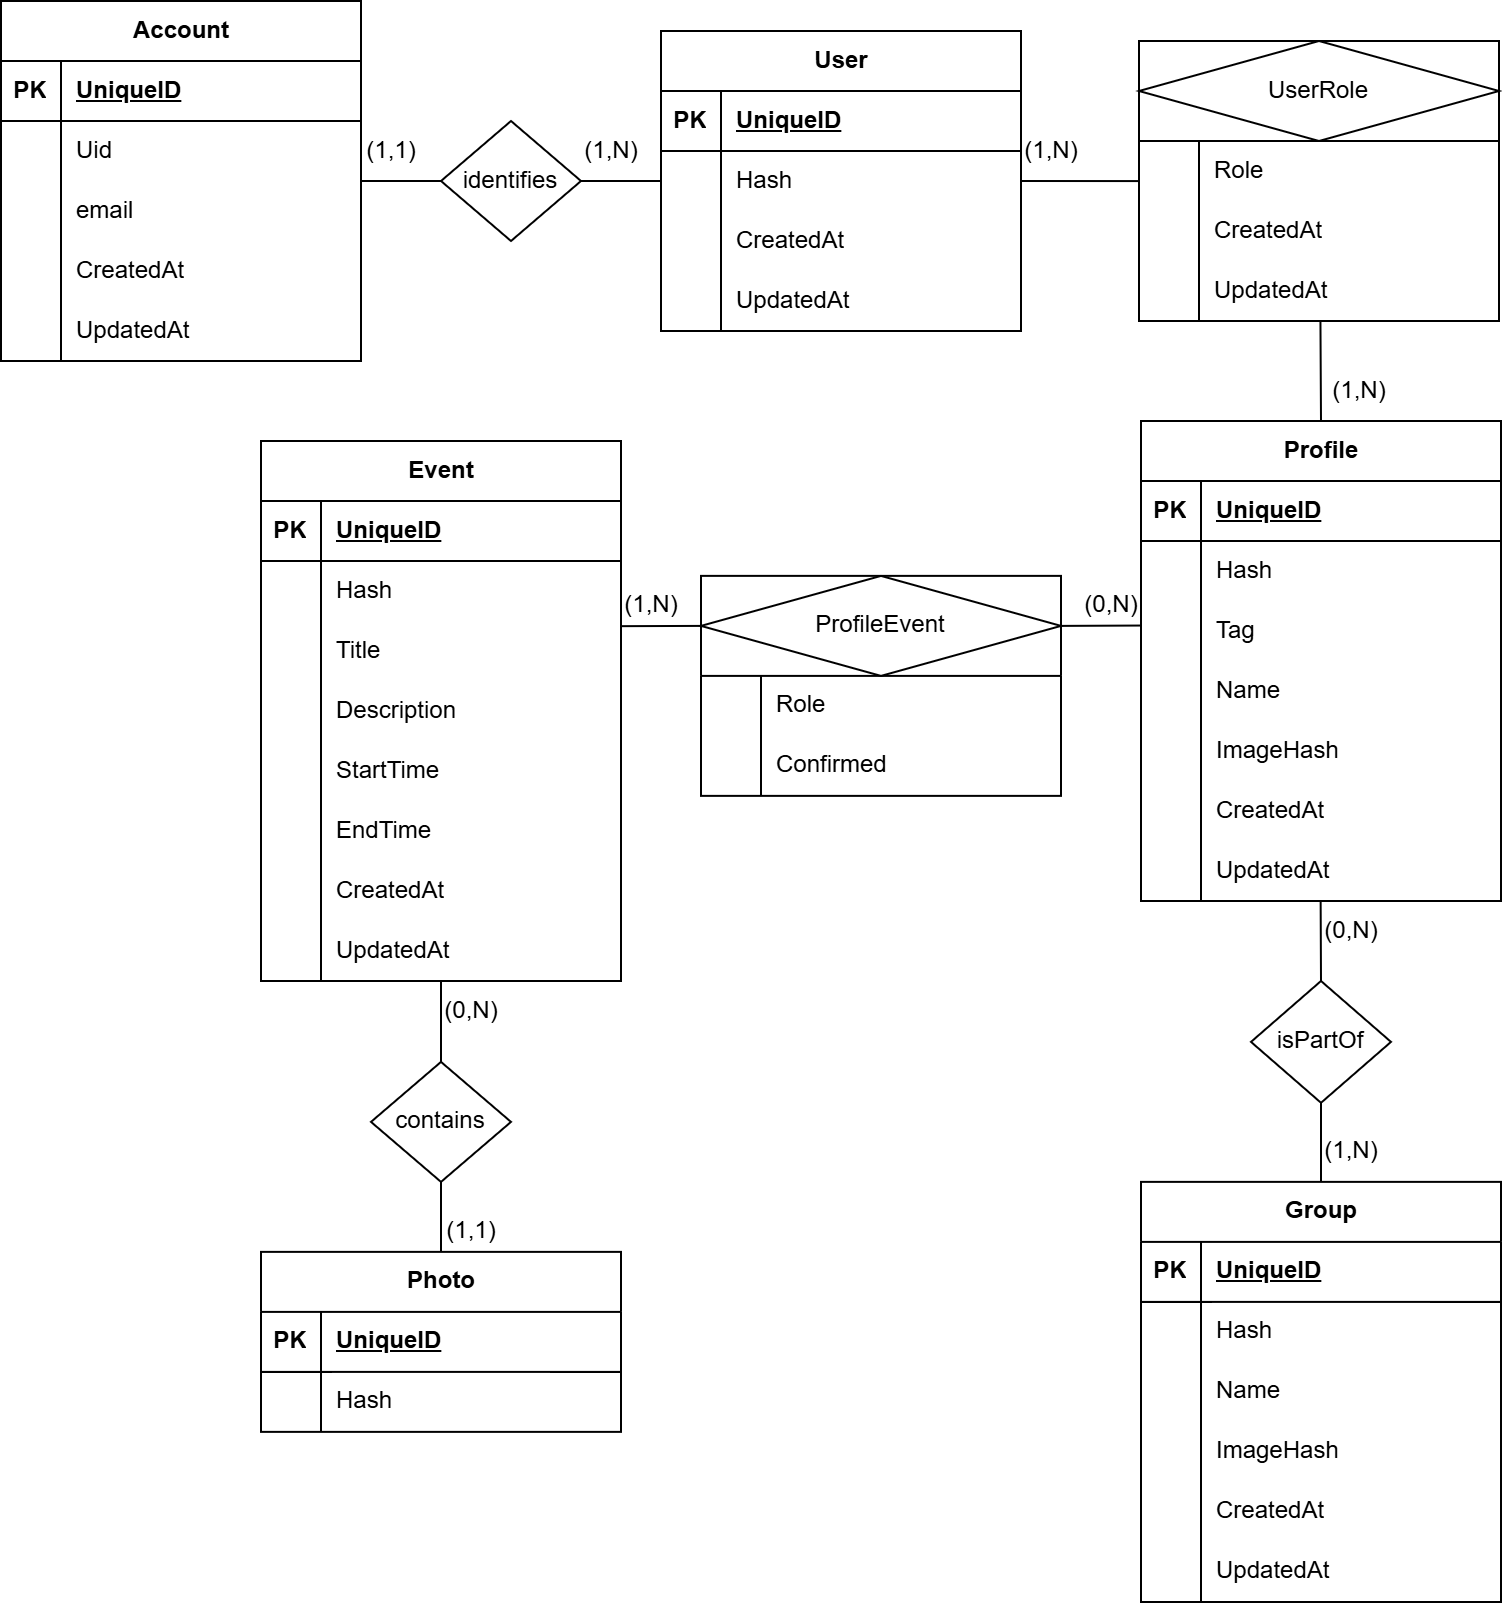
\includegraphics[width=\textwidth]{ProgettoDiagrammaER.png}
    \caption{Diagramma Entità - Relzione del dominio}
\end{figure}	

Si creano quindi sul server le classi logiche del programma, a partire dal dominio. 
Ogni classe corrisponde ad un oggetto del dominio, presentando i valori e le relazioni dei componenti come attributi dell’oggetto.\\
\\
Entity Framework Core di .Net(EFCore) è una libreria di C\# che permette di unire le classi logiche del programma alle tabelle del database. 
Fornisce un’astrazione logica del collegamento con il database e le richieste relative, fornendo una rappresentazione di alto livello delle connessioni sottostanti. \\
\\
Una volta collegato il server con il database tramite le stringhe di connessione salvate sull’Azure Key Vault, 
sono state definite le proprietà tra le varie entità, per poi inizializzare in automatico la struttura del database. 
Le modifiche alla struttura del database vengono infatti generate automaticamente da EFCore in seguito alla creazione o alla modifica degli attributi degli oggetti. 
Questo permette di star dietro agli aggiornamenti, generando e salvando le modifiche da applicare ad ogni modifica delle proprietà del dominio.\\
\\
\begin{figure}[h!]
    \begin{center}
        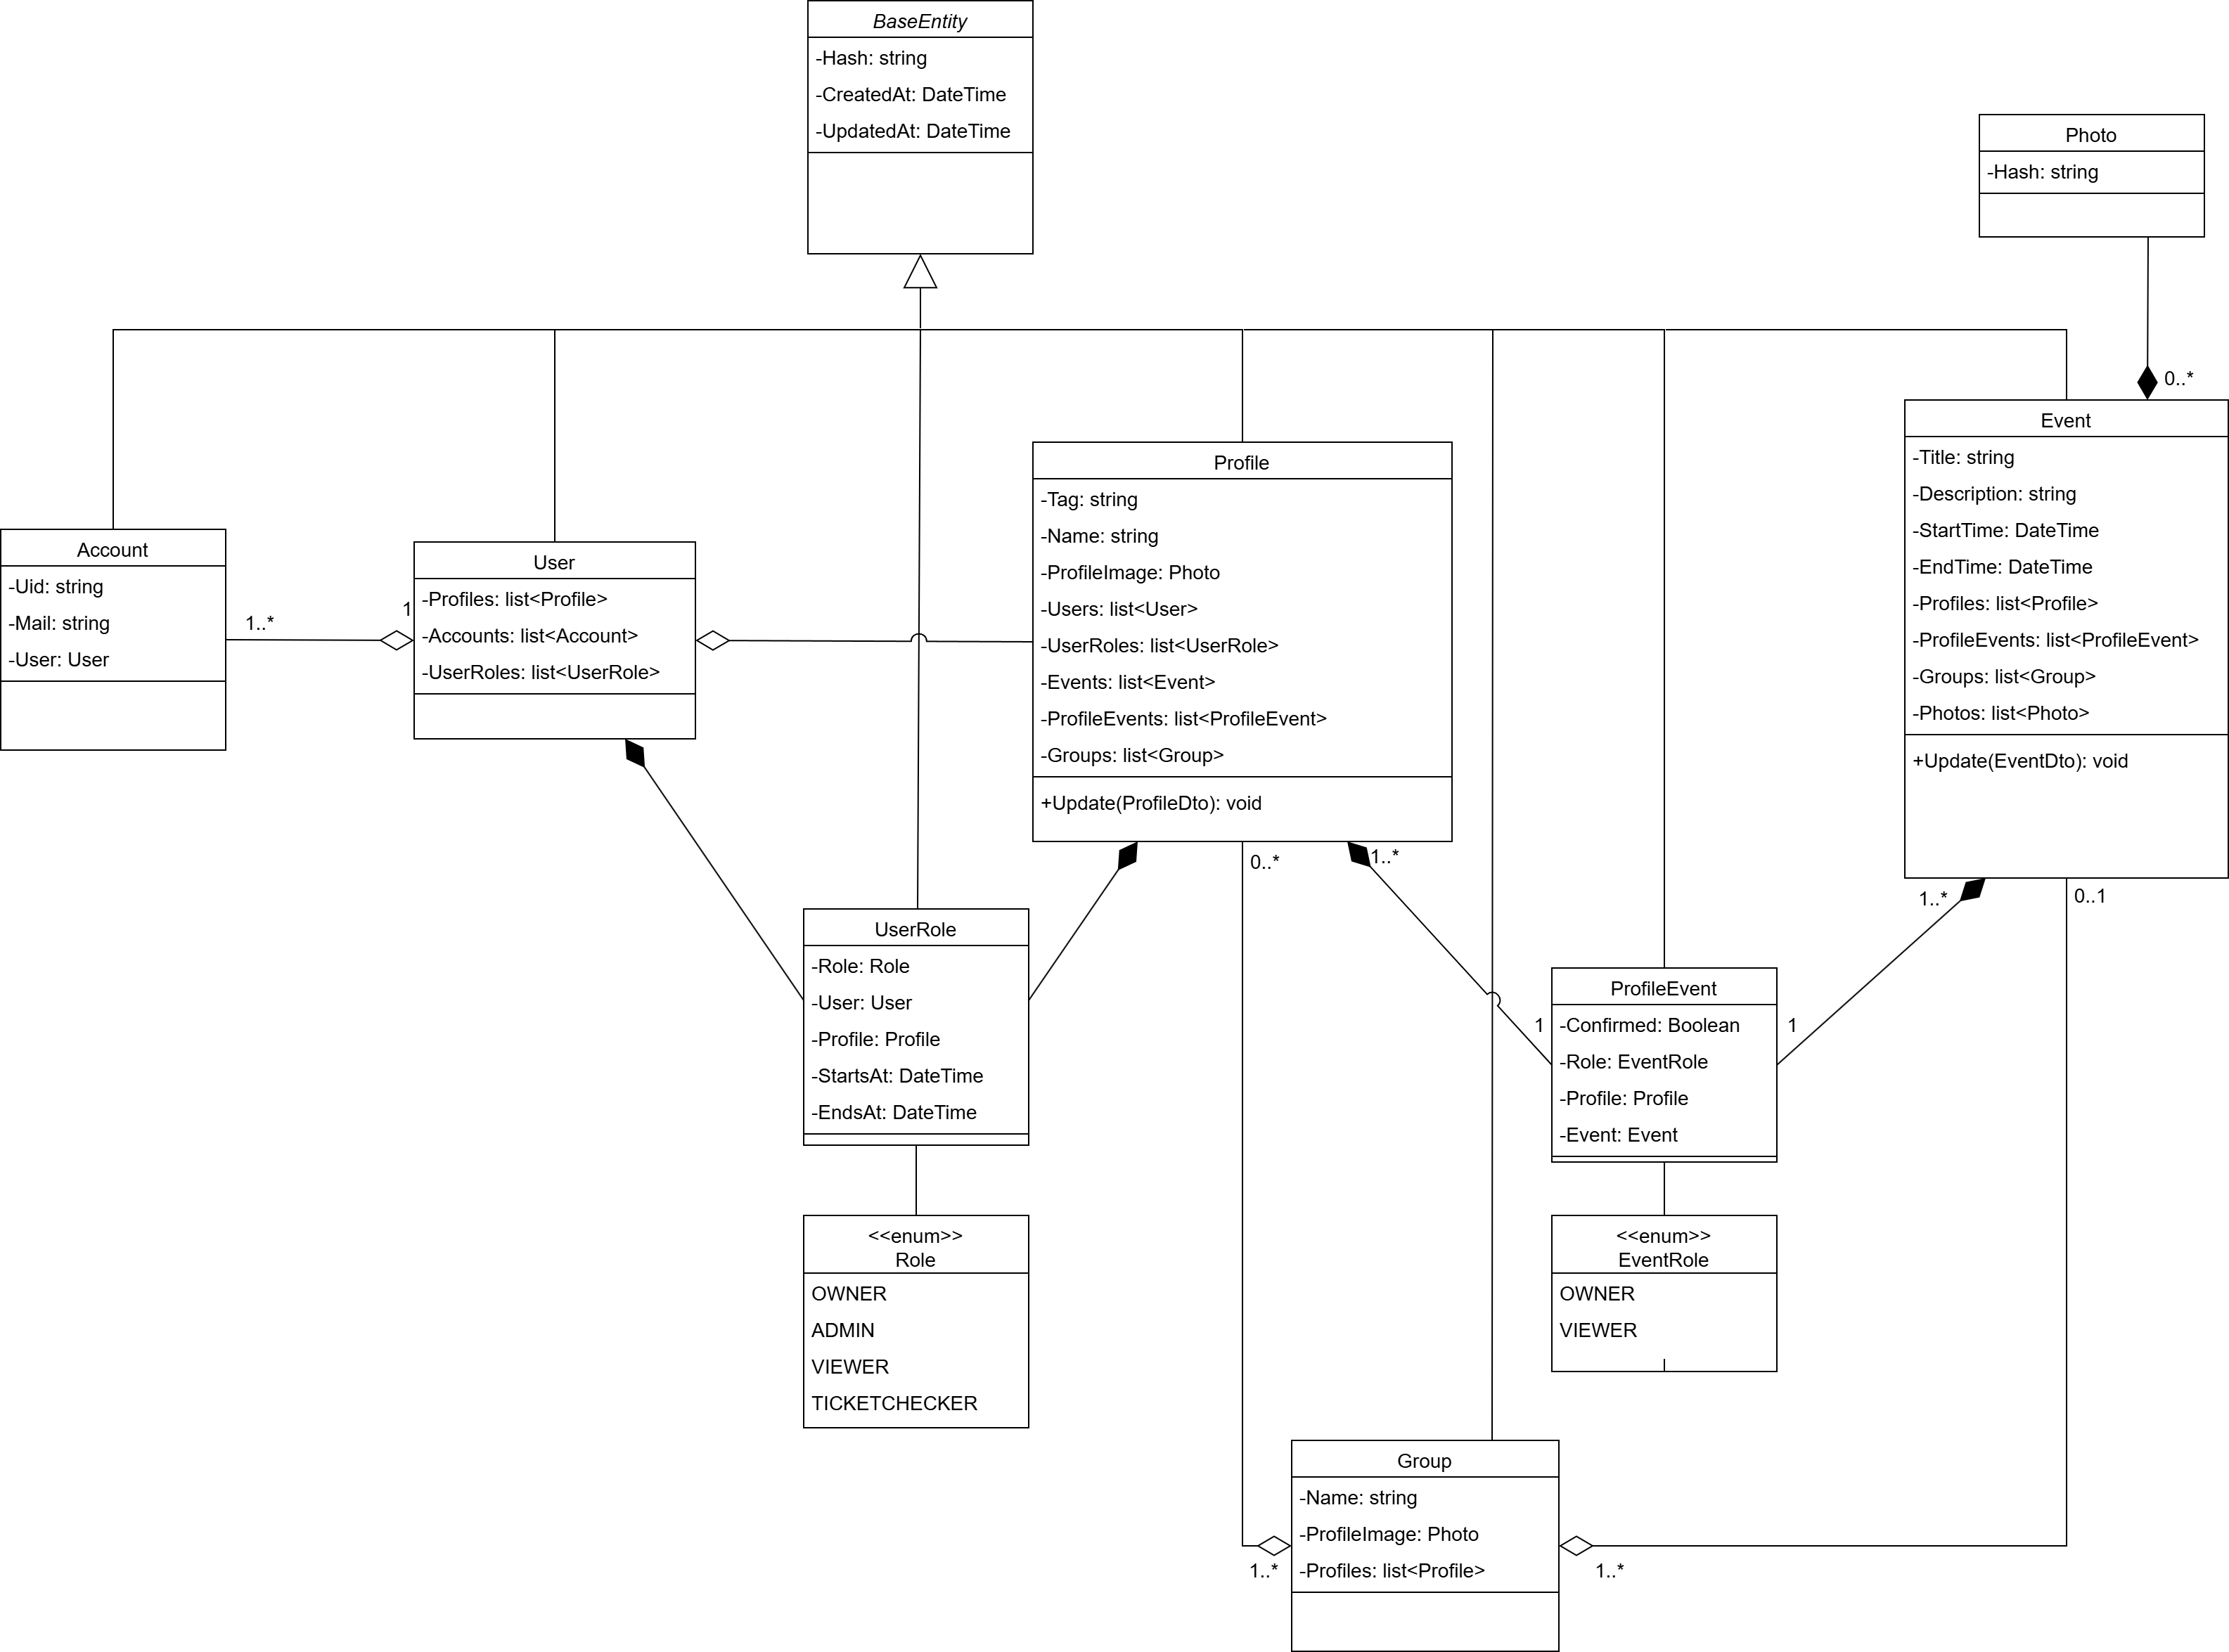
\includegraphics[width=\textwidth]{ModelClassDiagram.png}
        \caption{Modello delle classi del client}
    \end{center}
\end{figure}

Per la riduzione del carico computazionale richiesto da elementi con tante relazioni si utilizza la tecnica del lazy loading. 
La tecnica del Lazy Loading consiste nel richiedere i dati delle relazioni di un elemento solo quando strettamente necessario. 
La sua realizzazione tramite EFCore è attuata grazie alla proprietà virtual, 
che permette di gestire un oggetto con un riferimento al database richiedendo i dati delle sue relazioni solo quando viene espressamente richiesto.
\clearpage